\section{Project Code Structure}

The program has been written in python 3.6 and the list of dependencies can be found in the requirement.txt file. It is important 
to note that having a different version of python, keras, or tensorflow could result in runtime errors. Installing the tensorflow-gpu 
package greatly reduces the machine learning training time when compared to tensorflow-cpu.

The program has multiple independent modules that perform tasks:training, testing and scoring; that can be used to perform experiments 
for image localization. It also has the ability to automatically detect the environment:local, talapas and openstack; in which the code
 is running. Each module has a default set of parameters in a configuration file, which can be overridden by command line arguments 
 when running a module from the command line.

The file structure of the code can be seen in Figure \ref{fig:code_file_structure}. The main folders to focus on at the root level of the project are src and 
outputs. The source code is located inside the src folder and the output folder contains the results produced after running a module.

The src folder has 6 subdirectories $\colon$ architectures, $csv\_to\_image$, $patches$, $predictions$, $scoring$ and $shared$. The 
independently runnable 
modules are $csv\_to\_image$, $patches$, $predictions$, and $scoring$, whereas the other two folders, shared and architectures, are consumed by 
the other modules.

Each runnable module follows a convention for naming files and folders. The config folder contains json files- one per environment- that 
have default values numerous variables that are used in the code. A \emph{$config\_loader.py$} folder is also present in this folder, which parses 
command line arguments that can be passed as inputs to the module. These input values override the default values that are present in 
the json file. 

To run a module, the \emph{$<$module$\_$name$>$$\_$runner.py} file needs to be executed. The \emph{$<$module$\_$name$>$$\_$runner.srun} files store the 
configurations for submitting a job in talapas. Command line inputs need to be provided in the .srun file when the module is executed in talapas. 

The shared and architectures folders do not contain any files that can be executed independently. The architectures folder contains files
that must implement a method called get\_model, which should return a machine learning model object. Currently, only model objects from
the Keras and Sklearn libraries are returned. The shared folder contains files with static python classes that provide utility functions
and the name of the file indicates the type of utility functions it has.

\begin{figure}
    \centering
    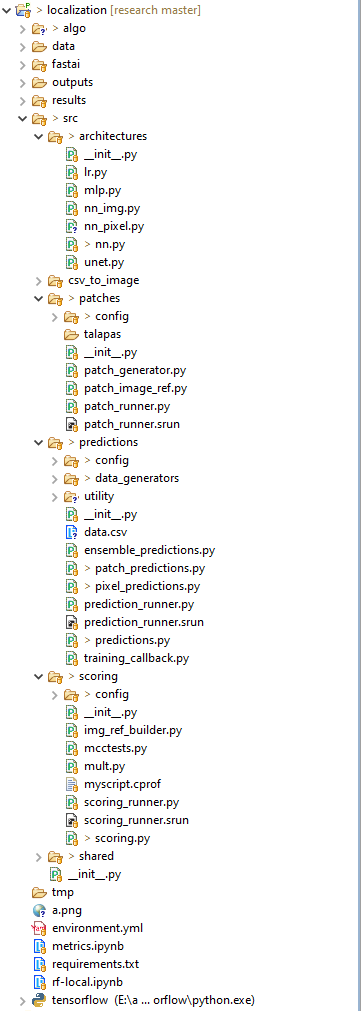
\includegraphics[width=\textwidth, height=0.9\textheight]
        {figures/code_file_structure.png}
    \caption{Code File Structure}
    \label{fig:code_file_structure}
\end{figure}
